\section{Results}

  \subsection{Three-Tone Shading}

    \begin{figure}
      \centering

      \subfloat[][]{
        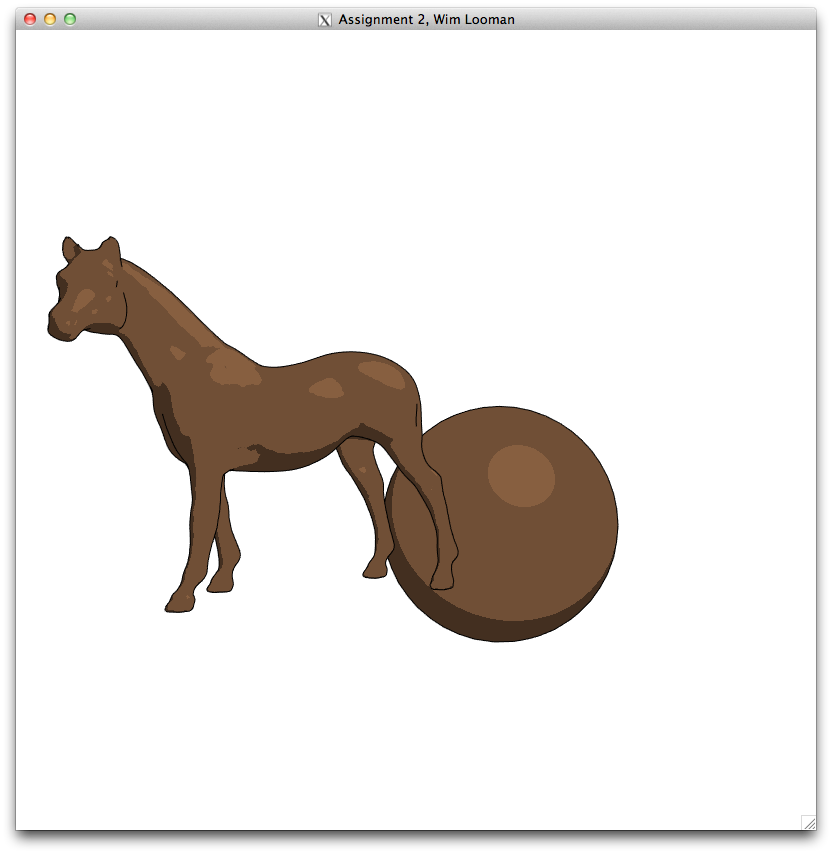
\includegraphics[width=0.45\textwidth]{images/three-tone-1}
      }

      \subfloat[][]{
        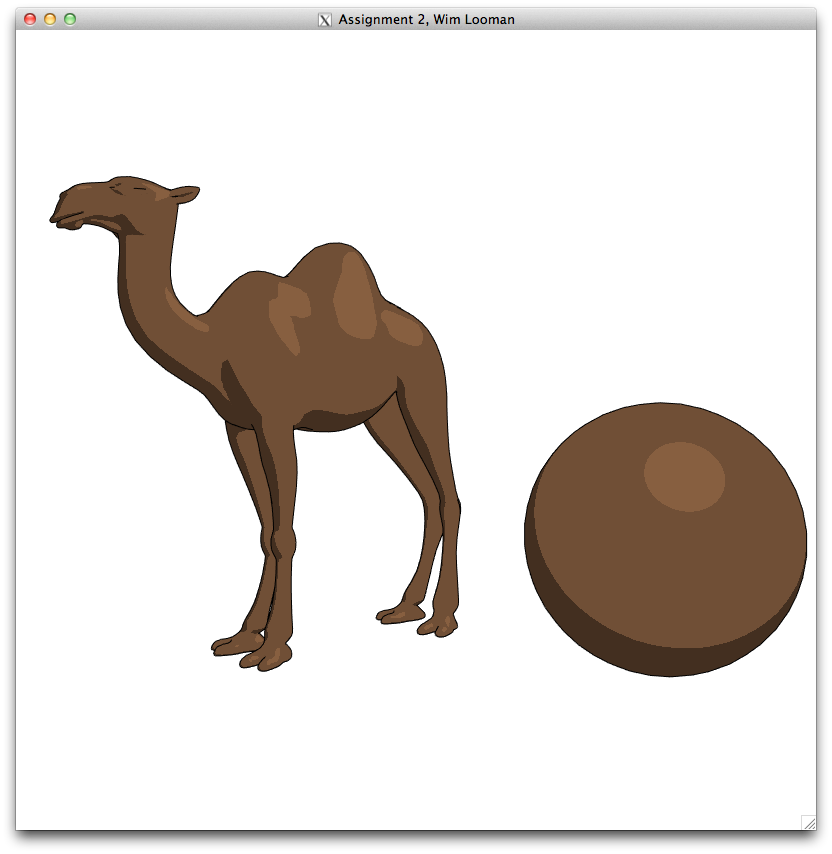
\includegraphics[width=0.45\textwidth]{images/three-tone-2}
      }

      \caption{Three tone-shading of three different models.}
      \label{three-tone}
    \end{figure}

  \subsection{Pencil Shading}
    \begin{figure}
      \centering

      \subfloat[][]{
        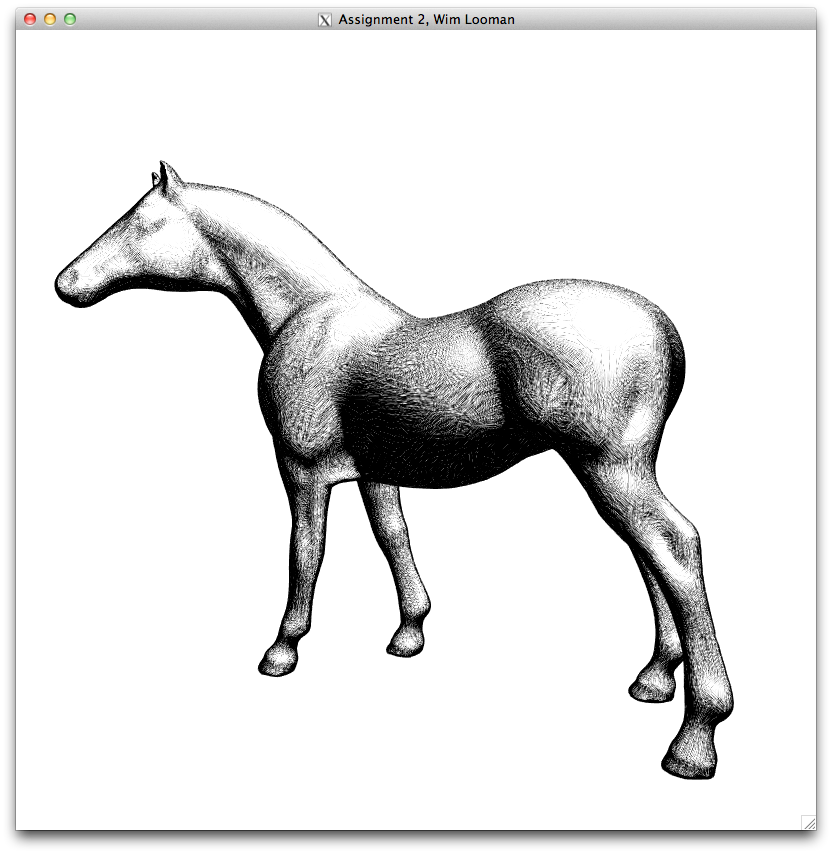
\includegraphics[width=0.45\textwidth]{images/pencil-1}
      }

      \subfloat[][]{
        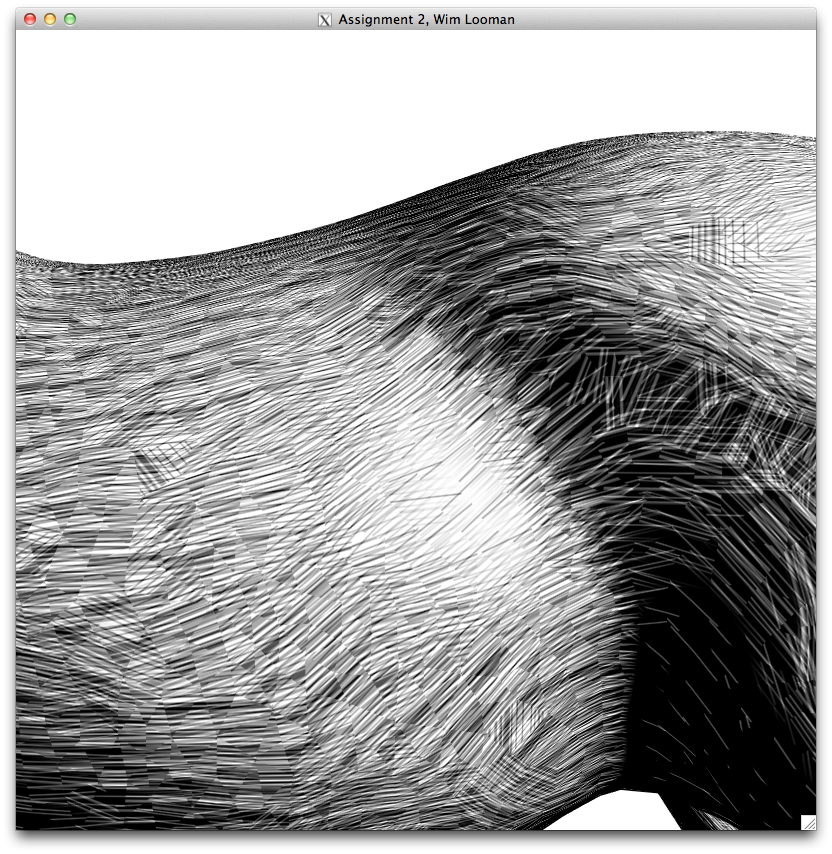
\includegraphics[width=0.45\textwidth]{images/pencil-2}
      }

      \caption{Pencil shading of horse model with close-up.}
      \label{pencil1}
    \end{figure}

    \begin{figure}
      \subfloat[][]{
        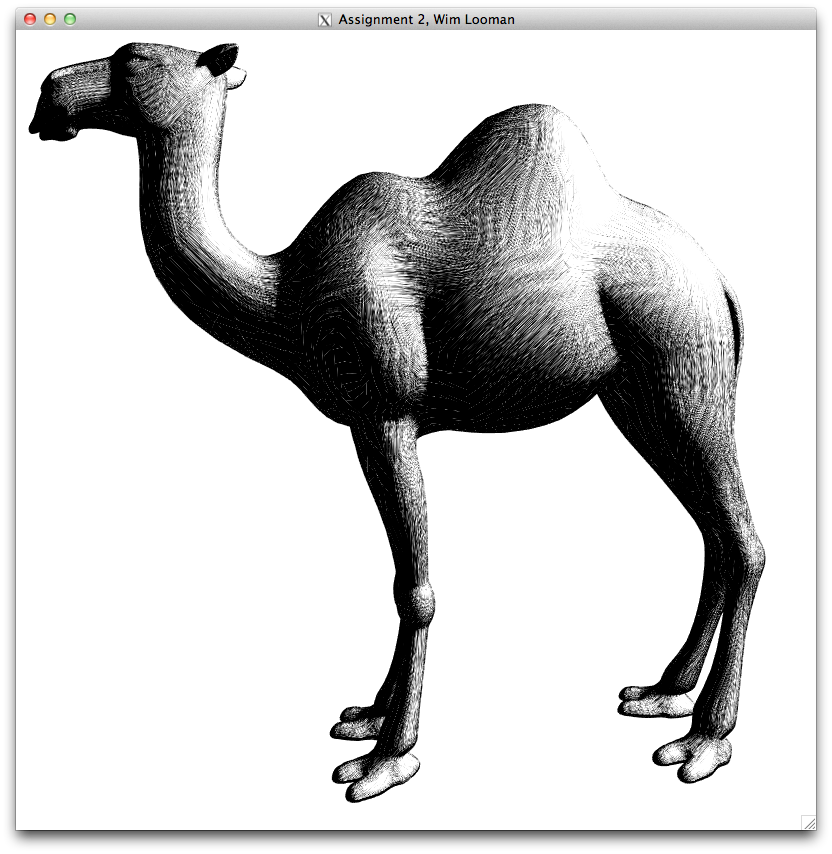
\includegraphics[width=0.45\textwidth]{images/pencil-3}
      }

      \subfloat[][]{
        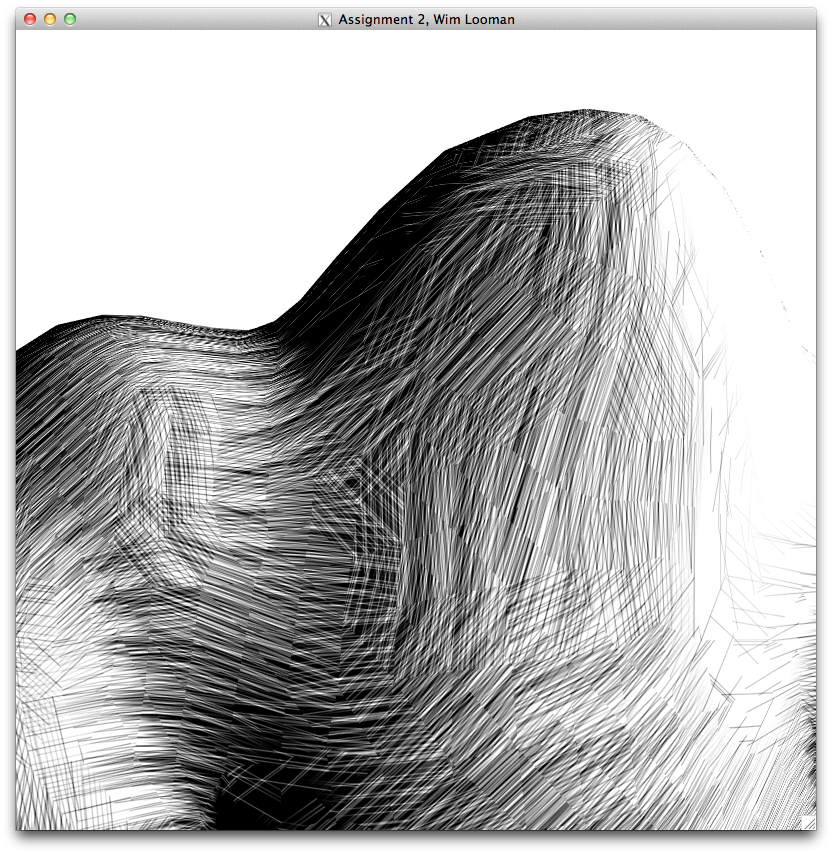
\includegraphics[width=0.45\textwidth]{images/pencil-4}
      }

      \caption{Pencil shading of camel model with close-up.}
      \label{pencil2}
    \end{figure}

